\chapter{L'interprétation}

\section{Introduction}
Nous avons vu que le $\lambda$-calcul utilise la réduction, basée sur un mécanisme de substitution.
Les langages interprétés que nous allons implémenter n'utilisent pas ce mécanisme de substitution, mais
font appel un environnement qui permet de représenter les paires variable/valeur.
A l'application d'une fonction, cet environnement est \textit{étendu} avec les nouvelles paires variable/valeur
des arguments de la fonction.

Nous perdons donc le côté  pur du $\lambda$-calcul qui se suffit à lui-même pour
dérouler ses calculs.
L'interprète ne pourra évaluer son expression qu'en présence d'un environnement.
Un interprète est ainsi  une fonction \verb+eval+ telle que \verb+(eval+ $\pi$ \verb+env)+ \imp\  \verb+valeur+

Nous reprenons ici  un peu du code de l'excellent blog :
\url{https://bernsteinbear.com/blog/lisp}.

Par rapport au code du blog cité, nous faisons deux changements majeurs. Le premier est d'utiliser à nouveau
les outils d'analyseur lexical et syntaxique \textbf{ocamllex} et \textbf{ocamlyacc}. 
Le second sera d'utilisé des listes mutables, afin de pleinement refléter toutes les capacités de Scheme qui n'est
pas un langage fonctionnel \textit{pur}.

Une fois cet interprète réalisé, nous l'utiliserons pour implémenter un nouvel interprète avec quelques variantes:
liaison \textit{dynamique} et \textit{statique}, évaluation \textit{stricte} et \textit{paresseuse} 
et enfin un interprète par \textit{continuation}, avant de conclure sur une tour de babel avec capacité de réification
et réflection de notre méta-interpète. C'est comme une quête philosophique\dots

Pour ces diffèrentes variantes, nous nous inspirons de notre bible sur le langage LISP : \textit{LISP In Small Pieces} de Christian Queinnec.
\cite{lisp}

\section{Un interprète \textsc{MiniScheme} avec \textsc{Ocaml}}

\subsection{L'évaluation}
Le $\lambda$-calcul repose sur un mécanisme de substitution permettant de réduire les termes et
aboutir à une forme normale. En programmation fonctionnelle, au lieu de réduire un terme, on
l'évaluera. Un terme non fermé ne pourra être évalué que dans un environnement où ses 
variables libres ont une liaison. Nous avons les définitions suivantes:
\begin{itemize}
	\item Une \textit{liaison} est un couple $(x,v)$ où $x$ est une variable et $v$ est une valeur.
	\item Un \textit{environnement} est une liste de liaison
	\item Une \textit{fermeture} est un couple $(M,\rho)$ où $M$ est un terme et $p$ un environnement 
	comportant une liaison pour chaque variable libre de $M$.
	\item Une \textit{valeur} est une fermeture $(M,p)$ avec $M$ de forme normale.
\end{itemize}
On formalise l'évaluation par la règle de jugement $\rho \vdash M \rightarrow v$. Elle exprime
que dans l'environnement $\rho$, le terme $M$ a pour valeur $v$.

La règle d'évaluation de l'appel par valeur se formalise ainsi comme suit:
\[(App_v): \frac{\rho \vdash M \rightarrow (\lambda x M^{'} , \rho ^{'} )  
		\ \ \ \ \ \rho \vdash N \rightarrow v \ \ \ \ \ (x,v);\rho ^{'} \vdash M^{'} \rightarrow v^{'} }
		 { \rho \vdash M N \rightarrow v^{'} }
\]

L'évaluation de $M^{'}$ le corps de la lambda se fait dans l'environnement $\rho ^{'}$ augmenté 
d'une liaison due du passage de paramètre. C'est la caractéristique de la liaison lexicale.
Pour  une liaison dynamique, l'évaluation du corps de la lambda se fera  dans l'environnement
courant $\rho$

Dans le cadre d'une implémentation en ML, l'erreur à ne pas faire (et que j'ai malheureusement faite initialement) est de
représenter la valeur d'une évaluation avec un type différent de l'expression à évaluer.
La puissance de Lisp repose sur  cette uniformité entre programmme et valeur. Nous utiliserons cette caractéristique pour
implémenter un interprète Lisp en Lisp.

Voici la séquence du code, depuis le stream en entrée de l'analyseur lexical jusqu'à la sortie de l'évaluateur \verb+eval+.
J'ai fait le choix d'avoir une représentation intermédiaire \verb+ast+ permettant de modéliser l'arbre syntaxique, et de faciliter
le processus d'évaluation.
\begin{center}
\begin{tikzpicture}
	\node (A) at (-1,0) {stream};
	\node (B) at (2,0) {token};
	\node (C) at (4,0) {\verb+exp+};
	\node (O) at (6,0) {};
	\node (P) at (6.5,1) {\verb+(if a b c)+};
	\node (Q) at (6.5,-1) {\verb+Paire(a, Nil)+};

	\node (D) at (7,3) {buildast};
	\node (M) at (13,0) {\verb+If(a,b,c)+};
	\node (E) at (10,0) {\verb+ast+};
	\node (F) at (7,-3) {eval};

	\tikzstyle{estun}=[->,>=latex]
	\draw[estun] (A)--node[above] {lex} (B);
	\draw[estun] (B)--node[above] {yacc} (C);
	\draw[estun] (C) to[bend left] (D) ;
	\draw[estun] (D) to[bend left] (E);
	\draw[estun] (E) to[bend left] (F) ;
	\draw[estun] (F) to[bend left] (C);

	\draw[dotted] (E) -- node {\textit{print}} (M) ;
	\draw[dotted] (C) -- node {\textit{print}} (P) ;
	\draw[dotted] (C) -- node {\textit{print}} (Q) ;
\end{tikzpicture}
\end{center}


Voici le code \textsc{Ocaml} des type abstrait \verb+exp+, \verb+ast+ et \verb+env+ :

\begin{Verbatim}
type exp =
| Booleen of bool
| Symbole of string
| Mot of string
| Entier of int
| Nil
| Paire of exp ref * exp ref
| Closure of string list * ast list * (env ref)
and ast =
| Atom of exp
| Var of string
| If of ast * ast * ast
| Cond of (ast * ast) list
| And of ast list
| Or of ast list
| Call of ast * ast list
| Call0 of ast    (* procedure sans argument *)
| Lambda of string list * ast list   
| Let of (string * ast) list * ast list
| Letrec of (string * ast) list * ast list
| Define of string * ast
| Begin of ast list
| Apply of ast * ast list
| Quote of exp
and env = (string * exp) list
  \end{Verbatim}


\subsection{Les étapes Read, Eval, Print}
L'interpr\'{e}te pr\'{e}sente trois \'{e}tapes que l'on d\'{e}crit souvent avec l'acronyme \textit{REPL} :
Read, Eval, Print, Loop


L'étape \textit{READ}  sera effectuée avec les moteurs ocamllex et ocmalyacc.
Cette étape va lire la saisie clavier et construire l'arbre syntaxique des expressions SCHEME.

Voici quelques exemples d'arbres syntaxiques générés avec Yacc.
Ces arbres syntaxiques sont à nouveau dessinés avec le package Tikz et nous avons développé une petite
fonction qui parcourt l'expression et génère le code Tikz.

\verb+(moins 4 3)+
\begin{center}
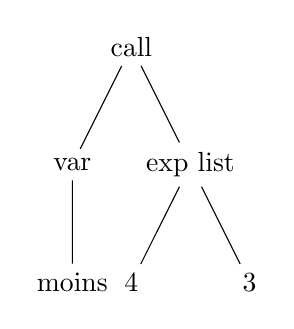
\begin{tikzpicture}[level distance=1.5cm]
\node {call} child {node {var} child { node{moins} }}  
             child {node {exp list} child { node {4 }}  child { node {3 } }}
;

\end{tikzpicture}
\end{center}


\verb+(if #t (plus 4 5) (moins 3 2))+
\begin{center}
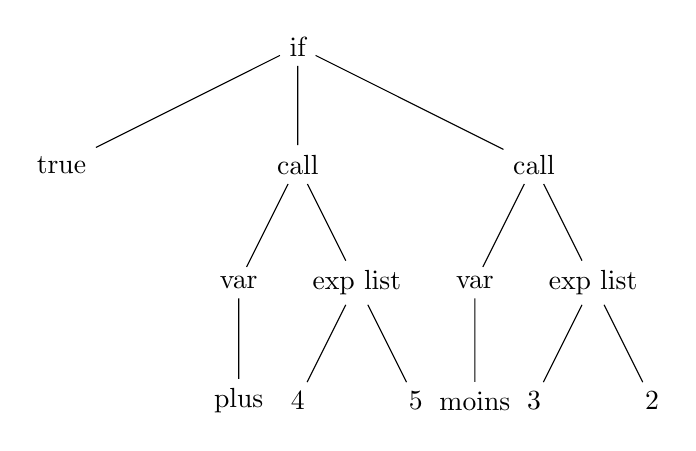
\begin{tikzpicture}[ level 1/.style={sibling distance=3cm},
level 2/.style={sibling distance=1.5cm},  level 3/.style={sibling distance=1.5cm}]

\node {if} child { node {true}}  child {node {call} child { node {var} child { node{plus} }}
child {node {exp list} child { node {4 }}  child { node {5 }} } }  child {node {call} child
{ node {var} child { node{moins} }}  child {node {exp list} child { node {3 }}  child { node {2 }} } }
;

\end{tikzpicture}
\end{center}

Et enfin une expression let \verb+(let ((a 2) (b 3)) (plus a b))+
\begin{center}
\begin{tikzpicture}[ level 1/.style={sibling distance=3.5cm},
level 2/.style={sibling distance=2cm},  level 3/.style={sibling distance=1.5cm}]
\node {let} child { child { node {bind} child { node{a }} child {node {2 }}}child { node {bind} child { node{b }}
 child {node {3 }}}} child {node {body let} child{node {call} child { node {var} child { node{plus} }}
   child {node {exp list} child { node {var} child { node{a} }}  child { node {var} child { node{b} }} } } } ;
\end{tikzpicture}
\end{center}

L'étape \textit{EVAL} va parcourir l'arbre syntaxique de l'expression, traiter cette expression et
en exprimer une valeur mod\'{e}lis\'{e}e avec le type \verb+value+

La fonction \verb+eval+ est une fonction prenant pour  arguments une expression de type \verb+ast+ et un environnement.
Elle retourne une valeur de type \verb+exp+. Voici sa signature: \\
\verb+val eval : ast -> env -> exp = <fun>+

L'étape \textit{PRINT} n'est autre que la fonction d'affichage finale de l'interpr\`{e}te.
Une fois cette étape finie, l'interprète boucle sur l'étape initiale \textit{READ}

\subsection{Liaison lexicale vs liaison dynamique}
Nous allons utiliser ici  la liaison lexicale (statique), et non dynamique.
 Cela nous impose de capturer l'environnement existant au moment de la d\'{e}finition de la fonction. 
Plus précisément, l'environnement est captur\'{e} par l'\'{e}valuation de la lambda, \'{e}valuation dont la valeur est appelée une \textit{closure}
ou \textit{fermeture}. 


\verb+ Lambda (parametres, expression) -> Closure (parametres, expression, env) +    


Dans le cas de la liaison dynamique, la fonction est appliqu\'{e}e en utilisant l'environnement courant, 
et non pas son environnement de définition. Donc pas besoin de fermeture.

A ma connaissance, la liaison statique est maintenant utilisée dans la plupart des langages fonctionnels.
En \sc{Scheme} et \sc{Ocaml},nous pouvons voir dans l'exemple ci-dessous que l'\'{e}valuation de la d\'{e}finition de la
 lambda \verb+inc_x+ capture la valeur de \verb+x+ .


\begin{tabular}{l|l} \hline
\sc{Scheme} & \sc{Ocaml} \\ \hline 
\verb!> (define x 1)! & \verb+# let x = 1+ ;; \\
\verb!> (define inc_x (lambda () (+ x 1)))! & \verb!# let inc_x = function () -> x+1 ;;! \\
\verb!> (inc_x)! & \verb!# inc_x ()! ;; \\ 
\verb!2! & \verb+- : int = 2+ \\
\verb!> (let ((x 100)) (inc_x))! &  \verb!# let x = 100 in inc_x () ;;! \\
\verb!2! & \verb+- : int = 2+  \\
\end{tabular}


\subsection{Gestion de l'environnement}


Comme indiqu\'{e} en pr\'{e}ambule, plusieurs choix sont possibles pour la mod\'{e}lisation de l'environnement.
Le choix le plus simple est une repr\'{e}sentation par une liste de paires $variable \leftrightarrow  value$
Ce choix peut être fait en OCAML par le type natif \verb+list+ ou en utilisant le type concret \verb+Paire of Symbole * lobject+

La principale difficulté est la représentation de fonctions récursives, comme en exemple la factorielle ci-dessous:
\begin{Verbatim}
(define fact 
 (lambda (n) 
  (if (eq? n 0) 
    1
    (* n (fact (- n 1)))))
\end{Verbatim}
Nous devons capturer l'environnement existant au moment de la définition de la fonction.
Cet environnement existant ne contient pas déjà la définition de \verb+fact+.

Il y a trois possibilités pour traiter ce problème de représentation d'un environnement \textit{récursif}.
\begin{enumerate}
  \item Utiliser une structure de liste qui permet à l'environnement capturé lors de la cloture de la lambda de boucler sur lui-même
La matérialisation de cette boucle ne peut à ma connaissance qu'être réalisée par un type liste \textit{mutable}.

Comment construire un environnement qui contient la fonction que l'on est en train de définir ?
\begin{Verbatim}
envRec =  (fac, <lambda corps>, envRec) :: env 
\end{Verbatim}
C'est une équation de point fixe\ldots

On remarquera également que le \verb+letrec+ de SCHEME peut être sémantiquement remplacé par un \verb+let+ associé de \verb(set!(
Et de la même manière, nous pouvons faire cette opération en ML, avec l'unique nuance est que le \verb+let+ temporaire représente bien
une fonction pour que la cohérence des types soit assurée.

\begin{Verbatim}
SCHEME
(letrec ((f e))
  corps)
  ==>
 (let ((f 'any))
    (let ((f-aux e))
       (set! f f-aux)
       corps))

(let ((fact 'any))
      (let ((f-aux (lambda (n) (if (eq? n 0) 1 (* n (fact (- n 1)))))))
        (set! fact f-aux))
  (fact 5))

OCAML 
let fact = ref (function x -> x) in
	let aux n = if n=0 then 1 else n * !fact (n - 1) in
	 fact:= aux ; !fact 5
\end{Verbatim}

  \item Dans le cas de fonction récursive, ne plus nous reposer sur l'environnement mais, comme en $\lambda$-calcul, 
  utiliser un combinateur de point fixe qui  permet de calculer le point fixe de notre fonction, sans avoir à la nommer.

  Nous allons utiliser ce procédé dans l'implémentation ML de notre interprète Scheme.

  Nous rappelons ci-dessous un exemple de  combinateur implémenté en SCHEME, et comment il peut être utilisé.
  \begin{Verbatim}
(define Y
(lambda(f)
 (let ((g (lambda (h) (lambda(x) ((f (h h) x))))))
  (g g))))

(define F*
  (lambda (f)
    (lambda (n)
      (if (eq? n 0)
          1
          (* n (f (- n 1)))))))
          
 (define fact (Y F*))
\end{Verbatim}
  
  \item La troisième approche est de modéliser l'environnement par une fonction, et non plus une liste d'association.
  La consultation de l'environnement consiste \`{a} appliquer la fonction \verb+env+ qui le repr\'{e}sente.

  Considérons l'expression \verb+(letrec ((x1 e1) ... (xn en)) corps)+  qui, on le rappelle, est \'{e}quivalente à 
  \verb+ ((lambda (x1 ... xn) corps) e1 ... en)+
  
  L'environnement capturé \verb+envRec+ au moment de la définition de la lambda  doit correspondre à 
  l'environnement étendu aux \verb+xi+ dont les valeurs sont données par l'évaluation des \verb+ei+ de la lambda 
  dans cet environnement \verb+envRec+
  C'est nécessaire afin que les \verb+ei+ puissent faire appel à des références récursives des \verb+xi+.
  
  Nous avons ainsi (et à nouveau) une équation de point fixe:
\[
  \begin{array}{l}
    envRec(x_i) = eval (e_i, envRec) \\
    envRec(x_i) = env (x_i) \ si \ x_i \notin letrec
  \end{array}
\]
  
\end{enumerate}

\section{Un interprète \textsc{Lisp} avec le nouvel interprète \textsc{MiniScheme} \ldots}
\subsubsection{La mise en abyme}

\begin{tabular} {lll}
  
\begin{minipage}{8cm}
    \textit{
      Pour obtenir cet effet, suivez-moi, j’invente un personnage de romancier, que je pose en figure centrale ;
      et le sujet du livre, si vous voulez, c’est précisément la lutte entre ce que lui offre la réalité et ce que,
       lui, prétend en faire.} \cite{gide}\\
       Les Faux-monnayeurs. André Gide\\
       
       \vspace{1cm}
       \textgreek{Kαὶ εἶπεν ὁ θεὸς πρὸς Μωυσῆν Ἐγώ εἰμι ὁ ὤν.}\\
       Exode 3, 14. La Septante
\end{minipage}

& \hspace{1cm}
&
\begin{minipage}{5cm}
    \begin{figure}[H]
      
\includegraphics[width=5.0cm]{gumpp.jpeg}
      \caption{Gumpp}
      \centering
    \end{figure}
    
\end{minipage}
\end{tabular}

 \subsubsection{\textsc{Lisp} mis en abyme} 
C'est ici un exercice assez classique.
Nous avons fait le choix d'un interprète avec liaison dynamique.
Nous aurons ainsi l'évaluation suivante retournant 13 et non 10.
\begin{Verbatim}
	((evaluate  
	'(let ((a 1))
	  (let ((f (lambda (b) (+ b a)))) 
		 (let ((a 3)) (f 10)))
	)) env)
\end{Verbatim}
En outre, il n'est pas nécessaire d'avoir un mécanisme de point fixe ou d'environnement récursif pour
l'appel d'une fonction récusrsive. C'est l'un des avantages de la liaison dynamique.
\begin{Verbatim}
((evaluate
 '(let ((fact (lambda (n) (if (= n 0) 1 (* n (fact (- n 1)))))))
   (fact 6)))
 env)
\end{Verbatim}


\section{L'auto-interprétation de l'interprète}
En rendant explicite la procédure \verb+eval+ et ses acolytes \verb+evlis, invoke, ...+ dans l'environnement
\verb+env+ , la procédure \verb+evaluate+ pourra être évaluée par elle-même. Le premier argument évalué de la fonction
est le symbole \verb+env+. Ce symbole devra être contenu dans l'environnement \verb+env+, c'est-à-dire dans lui-même\dots

Nous avons \verb+(eval '(eval '+$\pi$ \verb+ env) env)+ $\equiv$ 
 \verb+(evaluate '+$\pi$ \verb+ env)+ 

\subsection{La tour de Babel}

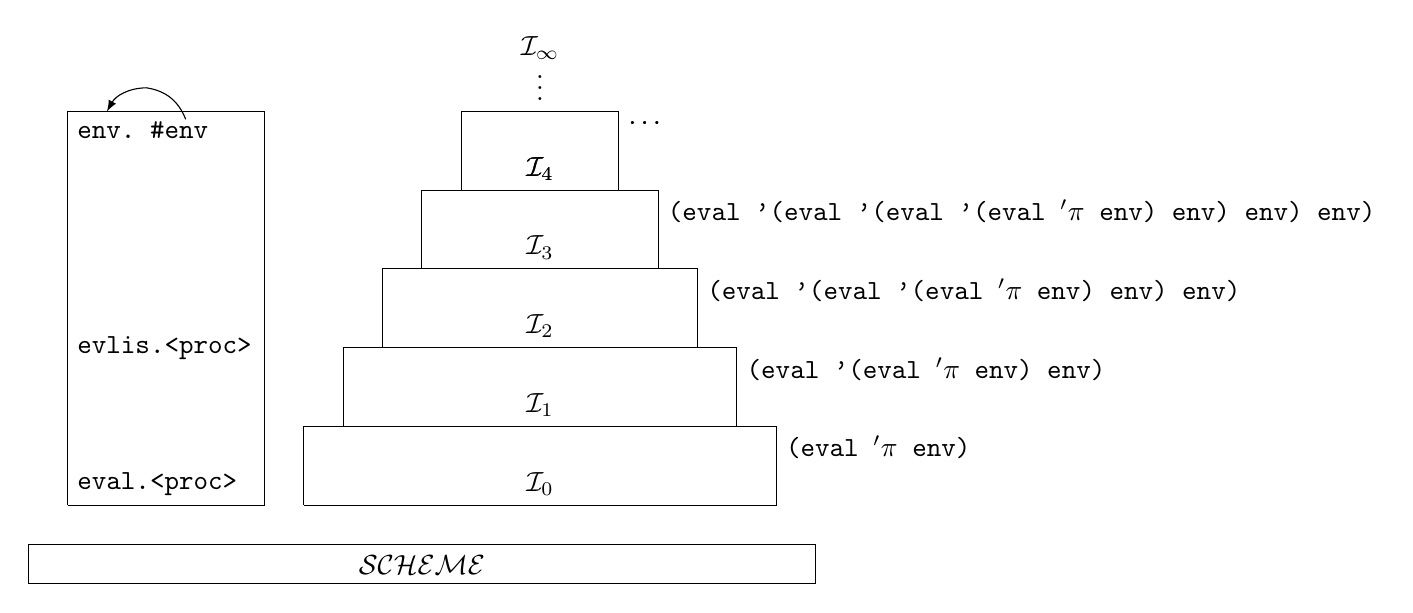
\begin{tikzpicture} 
%environnement

\tikzstyle{estun}=[->,>=latex]
\draw[estun] (-1.5,4.9) to [bend right] (-2, 5.3) to[bend right] (-2.5, 5) ;
\draw (-3, 0) node[above right]{\verb+eval.<proc>+}--(-0.5,0)--(-0.5,5)--(-3,5)
              node[below right]{\verb+env. #env+} --(-3,0) ;
    \node at (-3,2) [right]{\verb+evlis.<proc>+} ;

%the tower
  \draw (-3.5,-1)-- node[above]{$\mathcal{SCHEME}$} (6.5,-1) -- (6.5,-0.5)  -- (-3.5,-0.5) --(-3.5,-1) ;
	\draw (0,0)--node[above]{$\mathcal{I}_0$} (6,0) -- (6,1) node[below right]{\verb+(eval +$'\pi$\verb+ env)+}-- (0,1) -- (0,0) ;
	\draw (0.5,1)--node[above]{$\mathcal{I}_1$}(5.5,1) -- (5.5,2) node[below right]{\verb+(eval '(eval +$'\pi$\verb+ env) env)+}  -- (0.5,2) --(0.5,1) ;
	\draw (1,2)--node[above]{$\mathcal{I}_2$}(5,2) -- (5,3) node[below right]{\verb+(eval '(eval '(eval +$'\pi$\verb+ env) env) env)+} -- (1,3) --(1,2) ;
	\draw (1.5,3)--node[above]{$\mathcal{I}_3$}(4.5,3) -- (4.5,4) node[below right]{\verb+(eval '(eval '(eval '(eval +$'\pi$\verb+ env) env) env) env)+}-- (1.5,4) --(1.5,3) ;
  \draw (2,4)-- node[above]{$\mathcal{I}_4$} (4,4) -- (4,5) node[below right]{\ldots} -- (2,5) --(2,4) ;
  \draw (2,4)-- node[above]{$\mathcal{I}_4$} (4,4) -- (4,5) node[below right]{\ldots} -- (2,5) --(2,4) ;
  \node at (3,5.4) {\vdots} ;
  \node at (3,5.8) {$\mathcal{I}_\infty $} ;

\end{tikzpicture}

\begin{Verbatim}
	((evaluate (quote ((evaluate (quote ((evaluate (quote ((evaluate (quote (
		(lambda (x y) (+ x y)) (fact 5) (fact 6) )))
				   env))) env))) env))) env)
\end{Verbatim}

\subsubsection{L'environnement}
L'environnement doit contenir la valeur du symbole \verb+env+. Il doit faire référence à lui-même.
Seule une liste mutable peut modéliser cette boucle infinie. 
\begin{Verbatim}
> env ; affichage de l'environnement récursif avec DrRacket
#0=((env . #0#)
    (not . #<procedure:...interpreter2.scm:15:17>)
    (= . #<procedure:...interpreter2.scm:16:15>)
    (* . #<procedure:...interpreter2.scm:17:17>)
    (- . #<procedure:...interpreter2.scm:18:17>)
    (+ . #<procedure:...interpreter2.scm:19:17>)
    (atom? . #<procedure:...interpreter2.scm:20:19>)
    (boolean? . #<procedure:...interpreter2.scm:21:22>)
    (number? . #<procedure:...interpreter2.scm:22:21>)
    (cons . #<procedure:...interpreter2.scm:23:18>)
    (car . #<procedure:...interpreter2.scm:24:17>)
    (cdr . #<procedure:...interpreter2.scm:25:17>)
    (pair? . #<procedure:...interpreter2.scm:34:19>)
    (apply . #<procedure:...interpreter2.scm:36:22>)
    (fact . #<procedure:...interpreter2.scm:46:20>)
    (lookup . #<procedure:...interpreter2.scm:53:21>)
    (eprogn . #<procedure:...interpreter2.scm:63:21>)
    (evlis . #<procedure:...interpreter2.scm:74:20>)
    (invoke . #<procedure:...interpreter2.scm:85:14>)
    (extend . #<procedure:...interpreter2.scm:94:18>)
    (mapcar . #<procedure:...interpreter2.scm:105:18>)
    (mapcadr . #<procedure:...interpreter2.scm:113:19>)
    (evallet . #<procedure:...interpreter2.scm:121:6>)
    (evaluate . #<procedure:...interpreter2.scm:128:16>))
\end{Verbatim}

\subsection{Réification et réflexion}
La \textit{réification} est le fait de rendre concrète une chose abstraite.
Dans le cas de notre tour de Babel, réifier un objet du langage d'implémentation le rendra accessible au langage implémenté.
On peut citer l'exemple de la fonction \verb+eval+ rendant accessible dans Scheme le process d'évaluation. 
\verb+(eval '+$\pi$ \verb+) = + $\pi$

L'autre exemple que nous implémenterons est la réification de la continuation courante, mis à disposition
par la fonction \verb+call/cc+. Cette fonction prend en argument une lambda avec un seul paramètre qui récupère la
continuation courante de l'expression en cours d'évaluation.
\begin{Verbatim}
E = (e1 e2 ... (call/cc (lambda (k) ei)) ... en)	
\end{Verbatim}
  Si \verb+ei+ ne fait pas appel à \verb+k+, alors \verb+ei+ est évaluée normalement, ainsi que \verb+E+. 
Dans le cas contraire, \verb+k+ est appelée, liée à la continuation courante. Le résultat de \verb+ei+ est ainsi rendue
à cette continuation capturée \verb+(e1 ... [] ... en)+. Autrement écrit \verb+k = (lambda(v) (e1 ... v ... en))+
\begin{Verbatim}
(+ 5 (call/cc (lambda (k) (* 2 (k 8)))))  = 12
\end{Verbatim} 


L'environnement \verb+global-env+ partagé avec les différents interprètes $\mathcal{I}_i$ de notre tour de babel est aussi considéré
comme un environnement réifié. L'environnement du langage d'implémentation est ici mis à disposition aux langages implémentés.


La \textit{réflection} peut être vue comme l'opération inverse de la réification.
Elle permet la mise à disposition dans le langage d'implémentation un objet du langage implémenté.
Comme exemple, citons la fonction \verb+quote+ qui n'évalue pas son argument et le rend tel quel. \verb+quote+ est
 une primitive du langage Scheme dans le 
sens où il n'est pas possible  de redéfinir cette fonction avec les autre éléments du langage.
Avec l'implémentation de l'interprète $\mathcal{I}_R$ permettant les opérations de réflection et réification,
 cela deviendra possible. 

Pour faire court, la réflection est une opération d'abstraction ; la réification est l'application d'une abstraction.
Ce sont ainsi deux opérations réciproques. 
Voici ce que nous donne pour information la définition du terme \textit{abstraction} recherché dans notre dictionnaire.
\begin{definition}
  L'abstraction désigne le produit de l'opération qui consiste à isoler par la pensée une ou plusieurs qualités d'un objet
  concret pour en former une représentation intellectuelle
    
\end{definition} 

\vspace{0.5cm}

\begin{tabular}{c|c|c} \hline
réification & program vers data &  \verb+((reifier-to-cloture proc) (cdr e) r k)+   \\ \hline
réflection  & data vers program & \verb+(cloture-to-reifier (lambda (e r k) exp))+ \\ \hline
\end{tabular}


\subsubsection{L'interprète par continuation }
La fonction d'évaluation sera enrichie pour prendre trois arguments, le programme $\pi$ à évaluer, l'environnement 
$\rho$ et la continuation $\kappa$ 
\begin{center}
\verb+(eval+ $\pi\ \rho\ \kappa$ \verb+)+ \imp\  \verb+valeur+
\end{center}

Nous reprenons ici le code de l'excellent article \textit{a Simple Reflective Interpreter} \cite{reflective}
La fonction \verb+evaluate+ implémente un interprète Lisp en mode CPS de manière très naturelle.
La valeur ajoutée de l'article est la modélisation des fonctions. Trois types sont disponibles et 
distinguées par un tag dans l'environnement.
\begin{enumerate}
  \item Les fonctions utilisateurs \verb+(cloture (parl) exp env)+
  \item Les fonctions réifiées \verb+(reifier (e r k ) exp )+
  \item Les fonctions primitives \verb+(primitive nom )+
\end{enumerate}
L'application d'une fonction utilisateur se fait de manière classique par une évaluation du corps
de la lambda sur un environnement étendu aux nouvelles liaisons entre paramètres et arguments préalablement évalués.

Une fonction réifiée prend trois paramètres \verb+e+, \verb+r+ et \verb+k+.
\begin{itemize}
  \item  \verb+e+ est lié à la liste des arguments non évalués de l'application.
  \item \verb+r+ est lié à l'environnement de l'interprète évaluant l'application.
  \item \verb+k+ est lié à la continuation de l'interprète évaluant l'application.
\end{itemize}
Ainsi, nous avons un contrôle \textit{complet} de la fonction réifiée : contrôle du corps de la fonction et des arguments
non encore évalués par l'interprète sous-jacent, mais aussi la possibilité d'accéder à l'environnement et à la continuation
courante. En bref, no limit, on peut tout définir\dots

Les fonctions \verb+callcc+ et \verb+quote+ seront très simplement codées de la manière suivante:
\begin{Verbatim}
(define callcc (cloture-to-reifier (lambda (e r k) ((evaluate (car e) r id) k))))
(define quote (cloture-to-reifier (lambda (e r k) (k (car e) ))))
\end{Verbatim}


Dès le niveau 1 de notre tour, c'est-à-dire lorsque la fonction \verb+evaluate+ n'est plus évaluée par Scheme 
mais par elle-même, les formes spéciales \verb+if, quote, begin, define+ sont représentées par des fonctions réifiées.
La fonction d'évaluation peut ainsi être réduite à son strict minimum :
\begin{Verbatim}
(define evaluate
  (lambda (e r k)
    ((if (pair? e)
        (if (equal? (car e) 'lambda)
            eval-abstraction
            eval-application)
        (if (or (or (number? e) (string? e)) (boolean? e))
            eval-constante
            eval-variable))  
     e r k )))
\end{Verbatim}


\begin{minipage}{10.5cm}
  La fonction \verb+openloop+ peut être lancée à volonté et peut créer une succession 
  de  nouveaux étages dans notre tour de babel.
  Comme dans l'épisode biblique du livre de la Genèse\cite{genese}, 
  la faculté d'avoir un langage commun permet la construction
  d'une tour de hauteur potentiellement infinie.
   Nous nous retrouvons nous-même grisés par cette tour \textit{dont la tête touche les cieux}
  (\textgreek{ἡ κεφαλὴ ἔσται ἕως τοῦ οὐρανοῦ}). Nous citons ici la Septante (LXX).
  
  L'enthousiasme de pouvoir
  monter dans les étages doit cependant être tempéré. Le fait d'être à l'étage 
  $n+1$ n'apporte rien par rapport à l'étage $n$. L'application \verb+eval+ est idempotente car 
  $\forall \pi$ \verb+(eval '+$\pi$\verb+)+ $=$ \verb+(eval (eval '+ $\pi$\verb+))+.
  Autrement dit, la valeur \verb+(eval'+$\pi$\verb+)+ est un point fixe de \verb+eval+.
 

  \end{minipage}
  \hfill
  \begin{minipage}{5cm}
    \begin{figure}[H]
      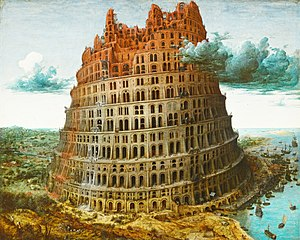
\includegraphics[width=5.0cm]{bruegel.jpg}
      \caption{Bruegel}
      \centering
    \end{figure}
    
\end{minipage}

\vspace{0.5cm}

\textgreek{ΓΕΝΕΣΙΣ     11 \\
  1. Καὶ ἦν πᾶσα ἡ γῆ χεῖλος ἕν, καὶ φωνὴ μία πᾶσιν. \\
   (...) \\ 
  9. διὰ τοῦτο ἐκλήθη τὸ ὄνομα αὐτῆς Σύγχυσις, ὅτι ἐκεῖ συνέχεεν κύριος τὰ χείλη πάσης τῆς γῆς.
}
\textit{\noindent
  Toute la terre avait alors une même parole ; il y avait une seule langue pour tous. \\ 
  À cause de cela, ce lieu fut appelé Babel (confusion), parce que là le Seigneur confondit les langues de toute la terre.
}

\vspace{0.3cm}
En pratique, malheureusement dès le niveau 3 de notre tour, les temps d'évaluation deviennent abominablement longs sur 
notre interprète  maison implémenté en OCAML.
Plusieurs minutes sont requises pour le calcul de la factorielle de cinq au niveau 3 de la tour.
C'est un peux plus rapide avec DrRacket, mais pas tellement. Le poids des sous-couches d'interprétation est lourd.
Dieu ne nous disperse pas ici par la confusion des langages, mais par la limitation de notre puissance de calcul \Laughey .


Voici le code complet de l'interprète au niveau 1. La fonction d'évaluation n'utilise pas ici
les réifications des fonctions \verb+if, quote, begin+.

\begin{footnotesize}
\begin{Verbatim}
(define evaluate
  (lambda (e r k)
    ((if (not (pair? e))
          (if (or (or (number? e) (string? e)) (boolean? e))
              eval-constante
              eval-variable)
          (if (equal? (car e) 'quote)
              eval-quote
              (if (equal? (car e) 'if)
               eval-if
                (if (equal? (car e) 'begin)
               eval-begin
               (if (equal? (car e) 'define)
                   eval-assign
                   (if (equal? (car e) 'lambda)
                       eval-abstraction
                       eval-application))))))
     e r k )))

(define eval-constante
  (lambda (e r k)
    (k e)))

(define eval-quote
  (lambda (e r k)
    (k (cadr e))))

(define eval-variable
  (lambda (e r k)
   (get-pair e r
   (lambda (success-pair)
    (k (cdr success-pair)))
    (lambda ()
    (wrong "symbol not bound " e)))))

(define eval-if
  (lambda (e r k)
    (evaluate (cadr e) r
              (lambda (v)
                (if v
                    (evaluate (caddr e) r k)
                    (evaluate (cadddr e) r k))))))

(define eval-assign
     (lambda (e r k)
       (evaluate (caddr e) r
                 (lambda (v)
                   (get-pair (cadr e) r
                             (lambda (success-pair)
                               (begin
                               (set-cdr! success-pair v)
                               (k (void)) ))
                             (lambda ()
                               (begin
                              (set-cdr! global-env (cons (car global-env)(cdr global-env)))
                              (set-car! global-env (cons (cadr e) v))
                              (k (void)))))))))

(define eval-define
  (lambda (e r k)
      (evaluate (caddr e) r
			(lambda (v) 
			(update! (cadr e) r v))))) 

(define eval-abstraction
  (lambda (e r k)
  (k (make-function (cadr e) (caddr e) r))))
					
(define get-pair
  (lambda (id r success failure)
    (find-pair id r
               success
               (lambda ()
                 (find-pair
                    id global-env success failure) )) ))

(define find-pair
  (lambda (elt alist success failure)
    ( (lambda (assq-result)
        (if assq-result
            (success assq-result)
            (failure)) )
      (assq elt alist) ) ) )

(define make-function
  (lambda (varl corps r)
     (list 'cloture varl corps r)))

(define eval-application
  (lambda (e r k)
       (evaluate (car e) r
              (lambda (proc)
                (if (equal? (car proc) 'reifier)
                    ((reifier-to-cloture proc) (cdr e) r k)
                    (evlis (cdr e) r
                       (lambda (args)
                         (apply-procedure proc args k))))))))

(define evlis
  (lambda (e r k)
    (if (null? e)
        (k '())
        (evaluate (car e) r
                  (lambda (v)
                    (evlis (cdr e) r
                           (lambda (w)
                            (k (cons v w)))))))))

(define eval-begin
  (lambda (e r k)
    (eprogn (cdr e) r k)))

(define eprogn
  (lambda (e r k)
   (if (null? (cdr e))
       (evaluate (car e) r k)
       (evaluate (car e) r (lambda (v)
                             (eprogn (cdr e) r k))))))

(define extend
  (lambda (env variables values)
        (if (or (null? variables) (null? values))
            env
            (cons (cons (car variables) (car values))
                  (extend env (cdr variables) (cdr values))))))
         
(define apply-procedure
  (lambda (proc args k)
    (if (equal? (car proc) 'cloture)
        (eprogn (list (caddr proc))
                (extend (cadddr proc) (cadr proc) args)
                k)
        (k (apply-primitive (cadr proc) args))))) 

(define apply-primitive
  (lambda (name args)
    (if (equal? name 'car)
        (car (car args))
     (if (equal? name 'or)
        (or (car args) (cadr args))
    (if (equal? name 'cdr)
        (cdr (car args))
    (if (equal? name 'cons)
        (cons (car args) (cadr args))
    (if (equal? name 'set-car!)
        (set-car! (car args) (cadr args))
    (if (equal? name 'set-cdr!)
        (set-cdr! (car args) (cadr args))
    (if (equal? name 'memq)
        (memq (car args) (cadr args))
    (if (equal? name 'assq)
        (assq (car args) (cadr args))    
    (if (equal? name '=)
        (= (car args) (cadr args))
    (if (equal? name '+)
        (+ (car args) (cadr args))
    (if (equal? name '-)
        (- (car args) (cadr args))
    (if (equal? name '*)
        (* (car args) (cadr args))
    (if (equal? name 'null?)
        (null? (car args))
    (if (equal? name 'not)
        (not (car args))    
    (if (equal? name 'symbol?)
        (symbol? (car args))
    (if (equal? name 'list)
        args
    (if (equal? name 'pair?)
        (pair? (car args))
    (if (equal? name 'read)
        (if (null? args) (read) (read (car args)))
    (if (equal? name 'eof-object?)
        (eof-object? (car args))
    (if (equal? name 'close-input-port)
        (close-input-port (car args))
    (if (equal? name 'newline)
        (newline)
    (if (equal? name 'equal?)
        (equal? (car args) (cadr args)) 
    (if (equal? name 'write)
        (write (car args))
    (if (equal? name 'display)
        (display (car args))
    (if (equal? name 'load)
        (load (car args)) 
    (if (equal? name 'number?)
        (number? (car args))   
    (if (equal? name 'string?)
        (string? (car args))   
    (if (equal? name 'boolean?)
        (boolean? (car args))   
     "erreur apply primitive"))))))))))))))))))))))))))))))

(define mapper
  (lambda (f l)
    (if (null? l)
        '()
        (cons (f (car l)) (mapper f (cdr l))))))

(define primitive-identifiers
  (lambda ()
    '(placeholder car cdr cons + - * = set-car! set-cdr! memq assq null? equal? newline  
      display read symbol? list pair? not load or number? string? boolean?)))

(define make-primitive
  (lambda (op)
    (list 'primitive op)))

(define reifier-to-cloture
  (lambda (reifier)
    (cons 'cloture (cdr reifier))))

(define cloture-to-reifier
  (lambda (cloture)
    (cons 'reifier (cdr cloture))))

(define make-reifier
  (lambda (formals body r)
    (list 'reifier formals body r)))

(define global-env '())

(define initialize-global-env
  (lambda ()
     (define global-env
      (extend global-env 
          (primitive-identifiers)
          (mapper make-primitive
                  (primitive-identifiers)))))) 

(define openloop
  (lambda (read-prompt write-prompt)
    (begin 
    (display read-prompt)
    (evaluate (read) '()
              (lambda (v)
                (begin
                (display write-prompt)
                (if (equal? v (void))
                  "rien a afficher"
                  (display v))
                (newline)
                (openloop read-prompt write-prompt)))))))

(define babel
  (lambda ()
       (begin
       (set-car! global-env (cons 'global-env global-env ))
       (openloop "i0 " "i0 "))))
\end{Verbatim}
\end{footnotesize}

